\documentclass{article}

% Cabecera del documento
% ======================================================================

% Paquetes extras
\usepackage[square, numbers, sort]{natbib}
% \usepackage{cite}
\usepackage{graphicx}
\usepackage{subcaption}
\usepackage[utf8]{inputenc}
\usepackage{amsmath,amssymb,amsfonts}
\usepackage{algorithmic}
\usepackage{textcomp}
\usepackage{float}
\usepackage{mathtools}
\usepackage[spanish]{babel}
\usepackage[paper=a4paper,margin=2.75cm]{geometry}
\usepackage{booktabs} % for tables
\usepackage{xurl}
\usepackage[colorlinks = true,
            linkcolor = blue,
            urlcolor  = blue,
            citecolor = orange,
            anchorcolor = blue]{hyperref} % for hyperlinks
\usepackage{xcolor} % text colors

% Directorio con imagenes
\graphicspath{{./figs/}}

% Cabecera del documento
% ======================================================================

% Titulo
\title{Diseño de controlador para sistema de Steering-by-Wire}

% Autores
\author{Rodrigo Aleo - 12106\\ aleorodrigof@gmail.com \\ \\ Control y Sistemas, Facultad de Ingeniería, \\ Universidad Nacional de Cuyo, \\ Mendoza, Argentina}

% Fecha
\date{Mayo de 2026, versión v2}

% Cuerpo del documento
% ======================================================================
\begin{document}

% Comandos definidos por el autor
\renewcommand{\tablename}{Tabla}
% \renewcommand{\color{blue}{#1}}{\azul}

% Crear cabecera
\maketitle

% Resumen
% ======================================================================
\begin{abstract}
    En este trabajo se desarrolla el modelado, control y validación por simulación de un sistema de dirección por cable aplicado al actuador del lado de las ruedas. La planta se formula en espacio de estados a partir de un modelo electromecánico que incluye la dinámica eléctrica del motor, la transmisión hacia la cremallera, la dinámica de la cremallera, el giro de las ruedas y perturbaciones asociadas a fricción y torque autoalineante. A partir del modelo lineal se verifican estabilidad, controlabilidad y observabilidad, y se diseña un controlador LQR para el seguimiento del ángulo de rueda. Como el controlador requiere realimentación completa de estados, se incorpora un observador de Kalman basado en la medición de posición lineal de cremallera, modelada con dinámica de sensor, muestreo, ruido y cuantización. También se analiza la selección de un actuador realista, adoptando un motor adecuado y validando sus límites de tensión, corriente, torque y velocidad. Finalmente, el modelo se evalúa ante perturbaciones representativas y se integra con un entorno de Unity para verificar cualitativamente la respuesta del vehículo usando entradas reales de volante. En conjunto, el trabajo permite validar la coherencia del modelo propuesto y evaluar las condiciones de operación del actuador en una arquitectura \textit{Steering-by-Wire}.
\end{abstract}

% Secciones
% ======================================================================
\section{Introducción}
\label{sec:intro}

% En la sección \ref{sec:intro}... 

En un sistema de direccionamiento de un automóvil convencional, el conductor induce en el volante una rotación que es transmitida mediante una conexión mecánica hacia las ruedas del automóvil. Una simplificación de dicho mecanismo puede observarse en la figura \ref{fig:sistemas_direccion}.

\begin{figure}[H]
    \centering
    \begin{subfigure}[b]{0.44\linewidth}
        \centering
        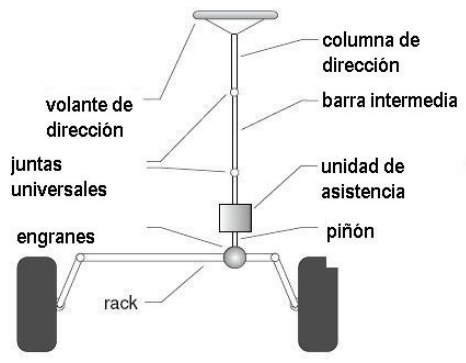
\includegraphics[width=\linewidth]{figs/Sistema de direccionamiento convencional.png}
        \caption{Sistema convencional}
        \label{fig:dir_convencional}
    \end{subfigure}
    \hfill
    \begin{subfigure}[b]{0.50\linewidth}
        \centering
        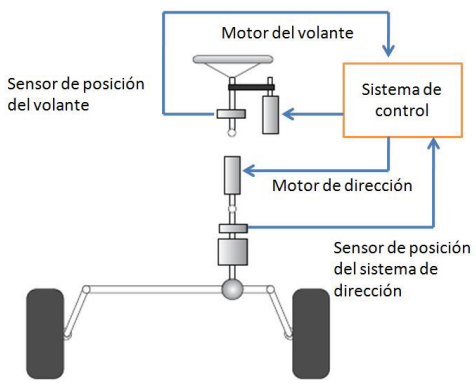
\includegraphics[width=\linewidth]{figs/SbW Modelo Sencillo.png}
        \caption{Sistema \textit{Steering-by-Wire}}
        \label{fig:dir_SbW}
    \end{subfigure}
    \caption{Comparación entre un sistema de direccionamiento convencional simplificado y una arquitectura \textit{Steering-by-Wire}.}
    \label{fig:sistemas_direccion}
\end{figure}

El sistema de \textit{Dirección por Cable} (\textit{Steering-by-wire} o \textit{SbW}) elimina la columna de dirección convencional que conecta el volante con el mecanismo de rotación de las ruedas, y la reemplaza por una interfaz completamente electrónica, como se ilustra en la figura \ref{fig:sistemas_direccion}. Un sensor de posición angular ubicado en el volante envía la señal a un controlador, el cual comanda un actuador electromecánico responsable del giro de las ruedas. Adicionalmente, puede integrarse un motor de retroalimentación en el volante que reproduzca las fuerzas generadas en las ruedas, con el objetivo de conservar la sensación de contacto con el terreno.

Como material ilustrativo del funcionamiento de este tipo de arquitecturas, pueden consultarse los videos \href{https://www.youtube.com/watch?v=f5GhTIMtr5I}{\textit{DIRECCION Por Cable: ¿Realmente Funciona? | Steer by wire}} y \href{https://www.youtube.com/watch?v=g1kp8ZzCnPI}{\textit{The Future of Steering Wheels: Is Steer-by-Wire the End of Traditional Steering? | Tech Explained}}.

Este enfoque constituye una innovación relevante en el ámbito automotriz, y presenta múltiples ventajas:

\begin{itemize}
    \item Reducción del peso y la complejidad del sistema, al eliminar componentes mecánicos.
    \item Mejora en la seguridad, al permitir que la dirección se integre con sistemas de control de tracción, estabilidad, frenado asistido, asistencia a la conducción y maniobras autónomas ante condiciones adversas.
    \item Posibilidad de modificar la relación entre el ángulo de giro del volante y el ángulo de las ruedas en función de la velocidad y otras variables, optimizando así la dinámica del vehiculo.
    \item Mayor flexibilidad en el diseño del habitáculo, al no requerir una conexión física entre el volante y el tren delantero.
\end{itemize}

Cabe destacar que en estos sistemas es de suma importancia la redundancia de los componentes críticos como son el actuador de dirección, sensores, cables que transportan señales y potencia eléctrica; todo con el fin de poder garantizar la seguridad de los tripulantes del vehiculo ante fallas en el sistema.

% ======================================================================
\section{Desarrollo}
\subsection{Modelado de la planta}
El sistema de direccionamiento de las ruedas consiste en un motor eléctrico que acciona la cremallera mediante una transmisión equivalente basada en husillo de bolas. En este tipo de actuador, la rotación del motor se convierte en desplazamiento lineal de la cremallera, la cual acciona las rótulas que permiten la rotación de las ruedas. En la figura \ref{fig:esquema_planta} puede verse una representación simplificada del sistema:
\begin{figure}[H]
    \centering
    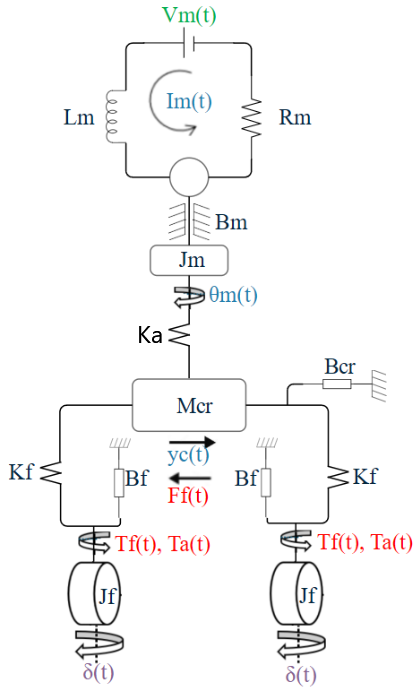
\includegraphics[width=0.3\linewidth]{figs/Esquema_planta.png}
    \caption{Esquema simplificado del sistema de dirección del tren delantero.}
    \label{fig:esquema_planta}
\end{figure}

Para formular el modelo se adopta la siguiente notación: $i_m(t)$ es la corriente del motor, $V_m(t)$ la tensión aplicada, $\theta_m(t)$ y $\omega_m(t)$ la posición y velocidad angular del eje motor, $y_c(t)$ y $v_c(t)$ la posición y velocidad lineal de la cremallera, y $\delta(t)$ y $\psi(t)$ el ángulo y velocidad angular de dirección de la rueda. Los parámetros físicos utilizados se resumen luego en la tabla \ref{tab:parametros_modelo}.

La ecuación eléctrica del motor se obtiene aplicando la ley de tensiones de Kirchhoff:
\begin{equation}
L_m \, \frac{di_m}{dt} = -R_m \, i_m(t) - K_e \, \omega_m(t) + V_m(t)
\label{ec_electrica}
\end{equation}

La conversión electromecánica se representa mediante las constantes $K_t$ y $K_e$, por lo que el torque desarrollado por el motor queda dado por $T_m(t)=K_t\,i_m(t)$. Para la transmisión por husillo de bolas se utiliza un radio cinemático equivalente $r_p$, calculado a partir del avance lineal por vuelta $p_{bs}$:
\begin{equation}
r_p = \frac{p_{bs}}{2\pi}
\label{ec_rp_ball_screw}
\end{equation}
De esta forma, la relación cinemática ideal entre el eje motor y la cremallera queda dada por $y_c(t)=r_p\,\theta_m(t)$.

La dinámica mecánica se obtiene aplicando las leyes de Newton al eje motor, a la cremallera y al giro de la rueda. Para el eje motor:
\begin{equation}
J_m \, \frac{d\omega_m(t)}{dt} = T_m(t) - B_m \, \omega_m(t) - K_{a} \left[ \theta_m(t) - \frac{y_c(t)}{r_p} \right]
\label{ec_motor}
\end{equation}

La ecuación dinámica de la cremallera es:
\begin{equation}
M_{cr} \, \frac{dv_c(t)}{dt} = -\frac{2 K_f}{r_l} \left[ \frac{y_c(t)}{r_l} - \delta(t) \right] - F_f(t) - B_{cr} \, v_c(t) + \frac{K_a}{r_p} \left[ \theta_m(t) - \frac{y_c(t)}{r_p} \right]
\label{ec_cremallera}
\end{equation}

Finalmente, la ecuación dinámica de cada rueda está dada por:
\begin{equation}
J_f \, \frac{d\psi(t)}{dt} = -K_f \left[ \delta(t) - \frac{y_c(t)}{r_l} \right] - B_f \, \psi(t) - T_f(t) - T_a(t)
\label{ec_rueda}
\end{equation}

En las ecuaciones anteriores, $K_a$ representa la rigidez equivalente de la transmisión entre motor y cremallera, mientras que $K_f$ representa la rigidez del enlace entre cremallera y ruedas. El factor $2$ en la ecuación de la cremallera contempla la contribución de ambas ruedas delanteras. Además, $r_l$ relaciona el desplazamiento lineal de la cremallera con el giro de rueda mediante $y_c(t)\simeq r_l\,\delta(t)$ para ángulos pequeños. Las perturbaciones externas se agrupan en la fuerza de fricción de cremallera $F_f(t)$, el torque de fricción de dirección $T_f(t)$ y el torque autoalineante del neumático $T_a(t)$.

En la tabla \ref{tab:parametros_modelo} puede verse un resumen de los parámetros que intervienen en el sistema, junto con los valores asignados.

\begin{table}[H]
\small
\centering
\caption{Parámetros del modelo de dirección por cable}
\label{tab:parametros_modelo}
\begin{tabular}{l l c c}
\toprule
\textbf{Símbolo} & \textbf{Descripción} & \textbf{Valor} & \textbf{Unidad} \\
\midrule
$L_m$     & Inductancia del motor & $0.42 \times 10^{-3}$ & $\mathrm{H}$ \\
$R_m$     & Resistencia del motor & $0.135$   & $\mathrm{\Omega}$ \\
$B_m$     & Fricción viscosa del motor & $1 \times 10^{-3}$ & $\mathrm{N \cdot m \cdot s / rad}$ \\
$J_m$     & Inercia del rotor & $1.0 \times 10^{-3}$ & $\mathrm{kg \cdot m^2}$ \\
$K_e$     & Constante contraelectromotriz & $0.6$     & $\mathrm{V \cdot s / rad}$ \\
$K_t$     & Constante de torque & $0.6$     & $\mathrm{N \cdot m / A}$ \\
$V_{m,\max}$ & Tensión máxima aplicada & $48$   & $\mathrm{V}$ \\
\midrule
$K_a$     & Rigidez del acoplamiento torsional & $3500$    & $\mathrm{N \cdot m / rad}$ \\
\midrule
$B_{cr}$  & Fricción viscosa de cremallera & $1.032$   & $\mathrm{N \cdot s / m}$ \\
$M_{cr}$  & Masa equivalente de cremallera & $2.0$     & $\mathrm{kg}$ \\
$r_l$     & Brazo cinemático rueda-cremallera & $0.115$   & $\mathrm{m/rad}$ \\
$p_{bs}$  & Avance del husillo de bolas & $32 \times 10^{-3}$ & $\mathrm{m/rev}$ \\
$r_p$     & Radio equivalente del husillo & $5.09 \times 10^{-3}$ & $\mathrm{m/rad}$ \\
\midrule
$B_f$     & Fricción viscosa de rueda & $30$      & $\mathrm{N \cdot m \cdot s / rad}$ \\
$K_f$     & Rigidez del enlace a rueda & $26000$   & $\mathrm{N \cdot m / rad}$ \\
$J_f$     & Inercia de giro de rueda & $0.270$   & $\mathrm{kg \cdot m^2}$ \\
\bottomrule
\end{tabular}
\end{table}

Los parámetros eléctricos y electromecánicos del motor se adoptaron a partir del \hyperlink{ref:mosrac-u13060}{catálogo del motor Mosrac U13060 de $48\ \mathrm{V}$}, utilizado como motor equivalente del actuador de ruedas. Los parámetros mecánicos de base del modelo de dirección por cable se tomaron como referencia del paper \hyperlink{ref:taher-2025}{\textit{Improving the Performance of Steering by Wire Using a Model Predictive Controller Enhanced with Particle Swarm Optimisation}}, y fueron ajustados para la arquitectura final con husillo de bolas.



Teniendo en cuenta las ecuaciones \ref{ec_electrica}, \ref{ec_motor}, \ref{ec_cremallera} y \ref{ec_rueda}, puede armarse el siguiente sistema de ecuaciones:


\begin{equation}
\left\{
\begin{aligned}
\frac{di_m(t)}{dt} &= \frac{1}{L_m} \,  \left[-R_m \, i_m(t) - K_e \, \omega_m(t) + V_m(t) \right] \\
\frac{d\theta_m(t)}{dt} &= \omega_m(t) \\
\frac{d\omega_m(t)}{dt} &= \frac{1}{J_m} \, \left\{T_m(t) - B_m \, \omega_m(t) - K_{a} \left[ \theta_m(t) - \frac{y_c(t)}{r_p} \right] \right\} \\
\frac{dy_c(t)}{dt} &= v_c(t) \\
\frac{dv_c(t)}{dt} &= \frac{1}{M_{cr}} \, \left\{ -\frac{2 K_f}{r_l} \left[ \frac{y_c(t)}{r_l} - \delta(t) \right] - F_f(t) - B_{cr} \, v_c(t) + \frac{K_a}{r_p} \left[ \theta_m(t) - \frac{y_c(t)}{r_p} \right] \right\} \\
\frac{d\delta(t)}{dt} &= \psi(t) \\
\frac{d\psi(t)}{dt} &= \frac{1}{J_f} \, \left\{ -K_f \left[ \delta(t) - \frac{y_c(t)}{r_l} \right] - B_f \, \psi(t) - T_f(t) - T_a(t) \right\}
\end{aligned}
\right.
\label{sistema_completo}
\end{equation}

El modelo de la planta se representa mediante un modelo lineal en espacio de estados:

\begin{equation}
\left\{
\begin{aligned}
\dot{x}(t) &= A \, x(t) + B_c \, u(t) + B_d \, d(t) ;\quad x(0) = \mathbf{0}\\
y(t) &= C \, x(t)
\end{aligned}
\right.
\label{ec_SS}
\end{equation}

Las variables de estado quedan definidas en el vector $x(t)$, y se relacionan entre sí mediante la matriz dinámica del sistema $A$:
\begin{equation*}
x(t) =
\begin{bmatrix}
i_m(t) &
\theta_m(t) &
\omega_m(t) &
y_c(t) &
v_c(t) &
\delta(t) &
\psi(t)
\end{bmatrix}^T
\end{equation*}

\begin{equation}
A =
\begin{bmatrix}
-\frac{R_m}{L_m} & 0 & -\frac{K_e}{L_m} & 0 & 0 & 0 & 0 \\
0 & 0 & 1 & 0 & 0 & 0 & 0 \\
\frac{K_t}{J_m} & -\frac{K_a}{J_m} & -\frac{B_m}{J_m} & \frac{K_a}{r_p\, J_m} & 0 & 0 & 0 \\
0 & 0 & 0 & 0 & 1 & 0 & 0 \\
0 & \frac{K_a}{r_p \, M_{cr}} & 0 & -\left(\frac{2\, K_f}{r_l^2} + \frac{K_a}{r_p^2} \right)\, \frac{1}{M_{cr}} & -\frac{B_{cr}}{M_{cr}} & \frac{2\, K_f}{r_l \, M_{cr}} & 0 \\
0 & 0 & 0 & 0 & 0 & 0 & 1 \\
0 & 0 & 0 & \frac{K_f}{r_l\, J_f} & 0 & -\frac{K_f}{J_f} & -\frac{B_f}{J_f} \\
\end{bmatrix}
\end{equation}

El vector de entradas de control $u(t)$ y su matriz $B_c$ son:
\begin{equation}
u(t) = V_m(t)
\end{equation}

\begin{equation}
B_c =
\begin{bmatrix}
\frac{1}{L_m} &
0 &
0 &
0 &
0 &
0 &
0
\end{bmatrix}^T
\end{equation}

El vector de entradas de perturbación $d(t)$ y su matriz $B_d$ son:
\begin{equation*}
d(t) =
\begin{bmatrix}
F_f & T_f & T_a
\end{bmatrix}^T
\end{equation*}

\begin{equation}
B_d =
\begin{bmatrix}
0 & 0 & 0 \\
0 & 0 & 0 \\
0 & 0 & 0 \\
0 & 0 & 0 \\
-\frac{1}{M_{cr}} & 0 & 0 \\
0 & 0 & 0 \\
0 & -\frac{1}{J_f} & -\frac{1}{J_f} \\
\end{bmatrix}
\end{equation}

Con respecto al vector de salidas $y(t)$ y su matriz correspondiente $C$, se tienen 2 versiones: una que se utiliza como salida de desempeño para el diseño del controlador, y otra que representa la variable medida por el sensor. La variable que interesa controlar es el ángulo de las ruedas $\delta(t)$. Por otro lado, el sensor mide la posición lineal de la cremallera $y_c(t)$, variable utilizada luego para el diseño del observador de estado. Por lo tanto:

\begin{equation}
y_p(t) = \delta(t) \, ; \quad C_p =
\begin{bmatrix}
0 & 0 & 0 & 0 & 0 & 1 & 0
\end{bmatrix}
\label{eq:salida_performance}
\end{equation}

\begin{equation}
y_s(t) = y_c(t)  \, ; \quad C_s =
\begin{bmatrix}
0 & 0 & 0 & 1 & 0 & 0 & 0
\end{bmatrix}
\end{equation}

\subsubsection{Limitaciones y simplificación del modelo}

A continuación se enumeran las principales simplificaciones y supuestos realizados en la construcción del modelo:

\begin{itemize}
    \item La planta utilizada para el diseño del controlador se modela como un sistema lineal e invariante en el tiempo (LTI), con parámetros constantes. Las saturaciones de tensión y los límites de operación del motor se consideran durante la simulación y validación del actuador, pero no forman parte de la matriz dinámica lineal $A$.

    \item Se considera que ambas ruedas delanteras giran con el mismo ángulo $\delta(t)$. Esta simplificación sigue al modelo cinemático tipo bicicleta. En la realidad, la geometría de dirección hace que las ruedas giren con ángulos distintos para respetar la condición de Ackerman. En la figura \ref{fig:modelo_ackerman} se ve un modelo cinemático que contempla este fenómeno:
    \begin{figure}[H]
        \centering
        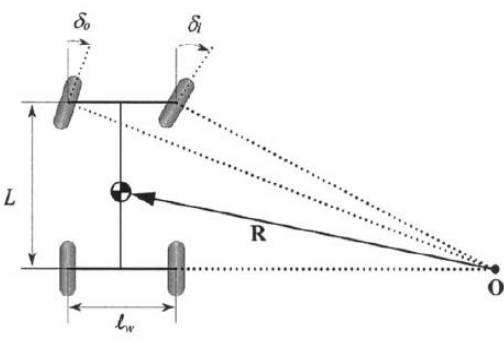
\includegraphics[width=0.4\linewidth]{figs/modelo_ackerman.png}
        \caption{Modelo cinemático de Ackerman}
        \label{fig:modelo_ackerman}
    \end{figure}

    \item El motor eléctrico se representa mediante un modelo continuo equivalente de corriente continua. No se modelan la conmutación electrónica, las fases del motor, el inversor ni el control PWM.

    \item No se consideran efectos eléctricos secundarios como inductancia mutua, histéresis magnética, saturación magnética ni corrientes parásitas. La conversión electromecánica se modela únicamente mediante las constantes $K_t$ y $K_e$.

    \item La transmisión motor-cremallera se representa mediante un radio cinemático equivalente $r_p$ asociado al husillo de bolas. No se modelan explícitamente la tuerca, el contacto entre bolas y pistas, la eficiencia variable, el juego mecánico ni posibles pérdidas internas del husillo.

    \item La elasticidad equivalente entre motor y cremallera se modela mediante un acoplamiento torsional con rigidez lineal $K_a$. No se incluyen deformaciones plásticas, rigidez no lineal ni modos flexibles de la transmisión.

    \item Las fricciones viscosas del motor, la cremallera y la rueda se incluyen dentro de la dinámica lineal. Las componentes secas o tipo Coulomb se representan como perturbaciones externas $F_f(t)$ y $T_f(t)$, por lo que no modifican la matriz $A$. Sus valores se consideran constantes y no se modela su variación con la velocidad, la temperatura ni el régimen de operación.

    \item Se adopta un enfoque de parámetros concentrados tanto para las masas como la rigidez mecánica. No se consideran efectos distribuidos ni modos flexibles.

    \item La carga sobre la cremallera se representa como una masa puntual con fricción viscosa y perturbación externa. No se modelan deformaciones locales, topes mecánicos ni límites de carrera dentro de la planta lineal.

    \item El torque autoalineante se incorpora como una perturbación externa $T_a(t)$. Su cálculo puede depender de variables no lineales del neumático, pero dicha no linealidad queda fuera de la matriz de estados de la planta.

    \item El sensor se modela fuera de la planta continua como una medición de posición de cremallera $y_c(t)$, con ruido, dinámica de primer orden y retención de orden cero en Simulink. La matriz $C_s$ solo representa qué variable de estado se mide.

    \item Se considera un único actuador de dirección, sin modelar la relación entre ambas ruedas ni la geometría completa de la dirección del vehículo.

    \item No se modelan elementos redundantes.
\end{itemize}

\subsubsection{Verificación con SimScape}
En la figura \ref{fig:simscape_vs_ss_diagrama} se ve cómo se llevó a cabo el diseño del sistema utilizando las herramientas de modelado de SimScape para utilizar de referencia y poder verificar si las ecuaciones para el sistema en espacio de estados han sido correctamente desarrolladas.

\begin{figure}[H]
    \centering
    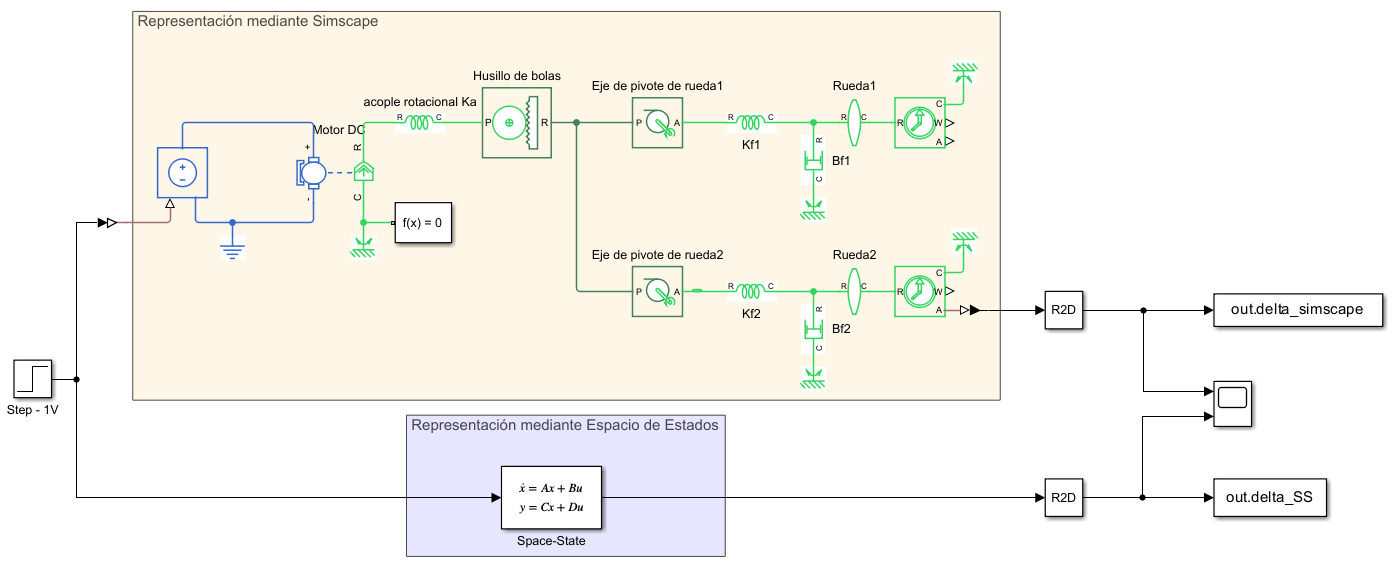
\includegraphics[width=1\linewidth]{figs/simscape_SS_diagrama.png}
    \caption{Diseño del modelo en SimScape y en Espacio de Estados}
    \label{fig:simscape_vs_ss_diagrama}
\end{figure}

\begin{figure}[H]
    \centering
    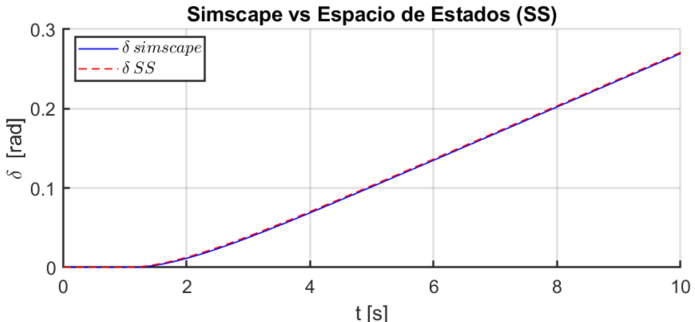
\includegraphics[width=0.6\linewidth]{figs/simscape vs SS.png}
    \caption{Variación de $\delta(t)$ con una entrada escalón $V_m = 1 \mathrm{V}$ }
    \label{fig:simscape_vs_ss}
\end{figure}

El resultado obtenido en ambos modelos es similar, y además es consistente con los resultados esperados, ya que al aplicar una entrada escalón de voltaje al motor, las ruedas deberían girar indefinidamente (sin considerar las limitaciones mecánicas en el rango de movimiento). Para este proyecto es de mayor conveniencia utilizar el sistema en espacio de estados debido a la facilidad que presenta para el diseño de controladores y observadores.

\subsubsection{Análisis de estabilidad}

Los polos de un sistema lineal expresado en espacio de estados pueden ser encontrados al calcular los autovalores de la matriz $A$, ya que estos representan la dinámica natural del sistema sin control. Se debe resolver la siguiente ecuación característica:

\begin{equation}
    \det(sI - A) = 0
\end{equation}

Al resolverlo de forma numérica en MATLAB se obtienen los siguientes polos:

\begin{table}[H]
\small
\centering
\caption{Polos del sistema de dirección por cable}
\label{tab:polos_modelo}
\begin{tabular}{c c}
\toprule
\textbf{Polo} & \textbf{Valor [$\mathrm{rad/s}$]} \\
\midrule
$p_1$ & $-0.4 + 8537.1i$ \\
$p_2$ & $-0.4 - 8537.1i$ \\
$p_3$ & $-141.4 + 943.8i$ \\
$p_4$ & $-141.4 - 943.8i$ \\
$p_5$ & $0$ \\
$p_6$ & $-75.2 + 286.3i$ \\
$p_7$ & $-75.2 - 286.3i$ \\
\bottomrule
\end{tabular}
\end{table}

Los polos del sistema se ubican todos en el semiplano izquierdo del plano complejo, con excepción de uno prácticamente nulo. Esto indica que el sistema es marginalmente estable. El polo $p_5 \approx 0$ corresponde a un modo integrador, lo cual se debe a una acumulación de estado sin disipación. Esto puede verse en la figura \ref{fig:simscape_vs_ss}, donde ante una entrada de tensión, el ángulo de las ruedas aumenta indefinidamente. Los polos $p_1$ y $p_2$ presentan una parte imaginaria elevada con poca atenuación, lo que refleja modos altamente oscilatorios de alta frecuencia asociados al sistema eléctrico. Por otro lado, los polos $p_6$ y $p_7$ representan modos más lentos, con menor frecuencia, que dominan la respuesta visible del sistema mecánico.

\subsubsection{Análisis de controlabilidad y observabilidad}

Un sistema en espacio de estados es completamente controlable si es posible llevar el estado desde cualquier condición inicial hasta cualquier otra en un tiempo finito mediante una entrada adecuada. Matemáticamente, esta condición se verifica a través del rango de la matriz de controlabilidad $\mathcal{C}$. Para este sistema de orden 7, considerando como entrada de control la tensión del motor $V_m(t)$, se define:

\begin{equation}
\mathcal{C} = \begin{bmatrix}
B_c & AB_c & A^2B_c & A^3B_c & A^4B_c & A^5B_c & A^6B_c
\end{bmatrix}
\end{equation}

Por otro lado, un sistema es completamente observable si, a partir de la evolución temporal de la salida medida, es posible reconstruir todos sus estados. En este modelo, la salida sensada es la posición lineal de cremallera $y_c(t)$, definida mediante la matriz $C_s$. La matriz de observabilidad $\mathcal{O}$ queda dada por:

\begin{equation}
\mathcal{O} = \begin{bmatrix}
C_s \\
C_sA \\
C_sA^2 \\
C_sA^3 \\
C_sA^4 \\
C_sA^5 \\
C_sA^6
\end{bmatrix}
\end{equation}

La verificación numérica se realizó evaluando el rango de ambas matrices con una tolerancia de $10^{-3}$. Para la controlabilidad desde la entrada $V_m(t)$ se obtuvo:

\begin{equation}
\mathrm{rank}\left(\mathcal{C}\right)=7
\end{equation}

Para la observabilidad desde la medición de cremallera $y_c(t)$ se obtuvo:

\begin{equation}
\mathrm{rank}\left(\mathcal{O}\right)=7
\end{equation}

Como ambos rangos coinciden con el orden del sistema, se concluye que la planta es completamente controlable desde la entrada $V_m(t)$ y completamente observable desde la medición de la posición de cremallera $y_c(t)$.

\subsection{Diseño de controlador}

Para el diseño del controlador se ha optado por la utilización del método LQR (Linear Quadratic Regulator). Este método busca minimizar la siguiente función de costo:

\begin{equation}
J \;=\; \int_{0}^{\infty}\bigl(x(t)^{T} \, Q_x \, x(t)\;+\;u(t)^{T} \, Q_u \, u(t)\bigr)\,dt
\end{equation}

La ley de control queda definida como:

\begin{equation}
u(t)\;=\;-K_{lqr}\,x(t)\;+\;k_{r}\,r(t)
\end{equation}

donde $K$ se obtiene resolviendo la ecuación de Riccati asociada y $k_{r}$ ajusta la ganancia de la referencia. La señal generada por esta ley de control se interpreta como la tensión que se desea aplicar al motor. Por este motivo, en la implementación de Simulink se limita la salida del controlador a $\pm48\ \mathrm{V}$ antes de enviarla al actuador y al observador. Esta saturación representa el límite de tensión del \hyperlink{ref:mosrac-u13060}{motor Mosrac U13060 de $48\ \mathrm{V}$} adoptado para el actuador de ruedas.

Se ha preferido LQR sobre un controlador PID por su capacidad de penalizar simultáneamente desviaciones de estado y esfuerzo de control, lo que facilita limitar la saturación del actuador y garantizar un compromiso óptimo entre desempeño transitorio y magnitud de la señal de control.

Lo realmente importante de este método es definir correctamente las matrices $Q_x$ y $Q_u$. En el modelo implementado, la salida de desempeño utilizada para el LQR es el ángulo de las ruedas delanteras:

\begin{equation}
y_p(t)=C_p\,x(t)=\delta(t).
\end{equation}

 La matriz $Q_x$ se construye a partir de la regla de Bryson aplicada a $\delta(t)$:

\begin{equation}
Q_y=\frac{\alpha_{\delta}}{\delta_{max}^{2}},
\qquad
Q_x=C_p^T\,Q_y\,C_p.
\end{equation}

La entrada de control corresponde a la tensión aplicada al motor, por lo que $Q_u$ se define como:

\begin{equation}
Q_{u} = \frac{\rho}{V_{m,\max}^2}
\end{equation}

Los coeficientes $\alpha_{\delta}$ y $\rho$ se eligen para equilibrar desempeño transitorio y magnitud de $u(t)$. Aumentar $\alpha_{\delta}$ exige con mayor rigidez el seguimiento de $\delta(t)$; aumentar $\rho$ penaliza más el uso de tensión del motor y suaviza la acción de control. En la tabla \ref{tab:valores_maximos_lqr} se definen los valores máximos usados para normalizar estas magnitudes.

\begin{table}[H]
\small
\centering
\caption{Valores máximos para variables de desempeño y entrada de control}
\label{tab:valores_maximos_lqr}
\begin{tabular}{c c}
\toprule
\textbf{Variable} & \textbf{Valor máximo} \\
\midrule
$\delta_{max}$ & $0.61 \; \mathrm{rad} \; = 35^\circ$ \\
$V_{m,\max}$ & $48 \; \mathrm{V}$ \\
\bottomrule
\end{tabular}
\end{table}

Luego de realizar varias pruebas, se optó por dar a los coeficientes los siguientes valores: $\alpha_{\delta}=1$ y $\rho=0.15$. Una vez definidas estas matrices, la ganancia de realimentación de estados se obtiene como:

\begin{equation}
K_{\mathrm{lqr}}=\mathrm{lqr}(A,B_c,Q_x,Q_u).
\end{equation}

Para seguimiento de referencia con el LQR puro se utiliza una ganancia de precompensación:

\begin{equation}
k_{r} = -\bigl(C_{p} \, (A - B_{c} \, K_{\mathrm{lqr}})^{-1} \, B_{c}\bigr)^{-1}.
\end{equation}

\begin{figure}[H]
    \centering
    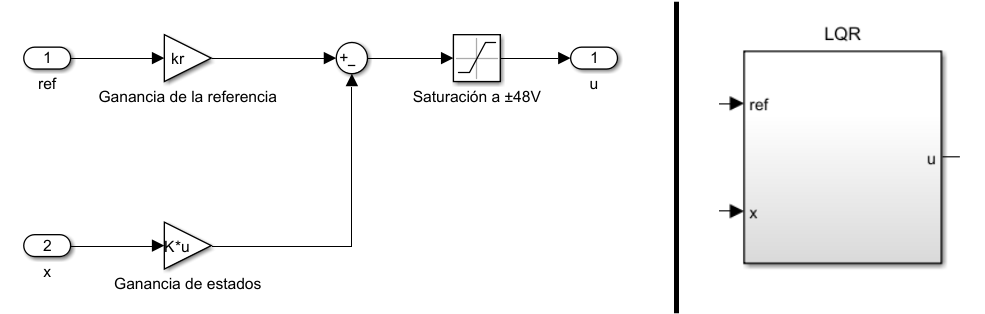
\includegraphics[width=1\linewidth]{figs/bloque_LQR.png}
    \caption{Bloque de controlador LQR en Simulink}
    \label{fig:bloque_LQR}
\end{figure}

\subsection{Limitaciones en el actuador}

Luego de limitar la señal de control a los valores admisibles del motor, el actuador de potencia se modela como una etapa ideal de modulación de tensión con ganancia unitaria. De este modo, la señal $u(t)$ entregada por el controlador se convierte directamente en la tensión aplicada al motor:

\begin{equation}
V_m(t)=u(t).
\end{equation}

Esta simplificación implica que no se modelan de forma explícita el inversor, el PWM, la dinámica interna del driver ni los retardos asociados a la electrónica de potencia. Los límites físicos del actuador se consideran previamente en la salida del controlador mediante la saturación de tensión, y luego se verifican junto con el resto de restricciones eléctricas y mecánicas del motor.

Los límites utilizados para validar la operación del motor se adoptan a partir del \hyperlink{ref:mosrac-u13060}{motor Mosrac U13060 de $48\ \mathrm{V}$}, utilizado como referencia del actuador equivalente. Estos valores se resumen en la tabla \ref{tab:limites_motor}.

\begin{table}[H]
\small
\centering
\caption{Límites de operación utilizados para validar el motor}
\label{tab:limites_motor}
\begin{tabular}{l c}
\toprule
\textbf{Magnitud} & \textbf{Límite adoptado} \\
\midrule
Tensión máxima $|V_m|$ & $48\ \mathrm{V}$ \\
Corriente continua $I_{\mathrm{cont}}$ & $30\ \mathrm{A}$ \\
Corriente pico $I_{\mathrm{peak}}$ & $70\ \mathrm{A}$ \\
Torque continuo $T_{\mathrm{cont}}$ & $18\ \mathrm{N\,m}$ \\
Torque pico $T_{\mathrm{peak}}$ & $40\ \mathrm{N\,m}$ \\
Velocidad nominal $|\omega_{m,\mathrm{nom}}|$ & $400\ \mathrm{rpm}$ \\
Velocidad máxima $|\omega_m|$ & $800\ \mathrm{rpm}$ \\
\bottomrule
\end{tabular}
\end{table}

\begin{figure}[H]
    \centering
    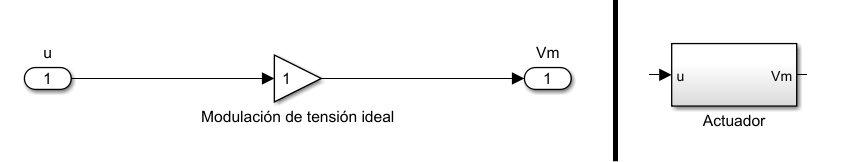
\includegraphics[width=0.9\linewidth]{figs/bloque_Actuador.png}
    \caption{Bloque de actuador con modulación ideal de tensión}
    \label{fig:bloque_Actuador}
\end{figure}


\subsection{Sensor}

El sensor utilizado en el modelo mide la posición lineal de la cremallera $y_c(t)$. Se descartó la alternativa de medir $\theta_m(t)$ con un encoder sobre el eje del motor debido a que este necesariamente realiza más de una revolución a lo largo de toda la carrera de la cremallera. En ese caso, un sensor angular absoluto de una sola vuelta no alcanza para reconstruir la posición absoluta de la cremallera sin agregar conteo de vueltas. Un encoder incremental sobre el motor también podría resolverlo, pero requiere conservar el conteo acumulado y gestionar fallas o reinicios. Por esta razón, para el observador resulta más simple medir directamente $y_c(t)$.

Se seleccionó como referencia el sensor \hyperlink{ref:mlx90513}{Melexis MLX90513}, un sensor inductivo automotriz para medición absoluta de posición rotativa o lineal.

El sensor está representado en Simulink mediante cuatro etapas. En primer lugar se modela la dinámica interna del sensor y el acondicionamiento de señal como un filtro pasabajos de primer orden:

\begin{equation}
y_{c,f}(s)=\frac{1}{\tau_{sensor} \, s+1}\,y_c(s)
\end{equation}

Luego, la señal filtrada se muestrea y se mantiene constante entre dos instantes consecutivos mediante una retención de orden cero. Sobre esa señal retenida se suma ruido discreto de medición $n[k]$, modelado como un error uniforme acotado, y luego se aplica cuantización con intervalo $q_{yc}$. Finalmente, la señal cuantizada es la medición entregada al observador en cada instante de muestreo.

Los parámetros adoptados para la simulación se muestran en la tabla \ref{tab:parametros_sensor}.

\begin{table}[H]
\small
\centering
\caption{Parámetros del sensor de posición de cremallera}
\label{tab:parametros_sensor}
\begin{tabular}{c c c}
\toprule
\textbf{Parámetro} & \textbf{Valor} & \textbf{Interpretación} \\
\midrule
$T_{s,sensor}$ & $0.01\ \mathrm{s}$ & período de actualización de la medición \\
$\tau_{sensor}$ & $0.001\ \mathrm{s}$ & constante de tiempo del filtro de primer orden \\
$e_{yc,\max}$ & $0.140\ \mathrm{mm}=1.40\times10^{-4}\ \mathrm{m}$ & error máximo de medición adoptado \\
$\sigma_{yc}$ & $0.081\ \mathrm{mm}=8.08\times10^{-5}\ \mathrm{m}$ & desviación estándar equivalente del error uniforme \\
$q_{yc}$ & $0.034\ \mathrm{mm}=3.42\times10^{-5}\ \mathrm{m}$ & intervalo de cuantización \\
\bottomrule
\end{tabular}
\end{table}

El datasheet del \hyperlink{ref:mlx90513}{Melexis MLX90513} especifica un error máximo de $\pm 0.1\%$ del fondo de escala. Considerando la carrera de cremallera utilizada en el modelo, $L_{yc}=140\ \mathrm{mm}$, dicho error equivale a:

\begin{equation}
e_{yc,\max}=0.001\,L_{yc}=0.001\, 140\ \mathrm{mm}
=0.140\ \mathrm{mm}=1.40\times10^{-4}\ \mathrm{m}.
\end{equation}

Además, en la tabla de especificaciones eléctricas se indica un ruido RMS de la señal de posición de $0.070^\circ_{\mathrm{el}}$ para la configuración menos favorable. Se utilizan grados eléctricos porque el sensor mide la fase de un sistema inductivo. En una aplicación lineal, dicha fase se calibra contra la carrera mecánica medida. Si se considera una calibración lineal de una vuelta eléctrica sobre la carrera útil de la cremallera, el ruido RMS equivalente resulta:

\begin{equation}
\sigma_{yc,\mathrm{RMS}}\simeq
\frac{0.070^\circ_{\mathrm{el}}}{360^\circ_{\mathrm{el}}}\,L_{yc}
=
\frac{0.070^\circ_{\mathrm{el}}}{360^\circ_{\mathrm{el}}}\, 140\ \mathrm{mm}
=0.027\ \mathrm{mm}=2.72\times10^{-5}\ \mathrm{m}.
\end{equation}

Sin embargo, para modelar el sensor se usa el error máximo $e_{yc,\max}=0.140\ \mathrm{mm}$, ya que este valor contempla no solo el ruido aleatorio sino también no linealidades (térmicas y magnéticas), errores de calibración y efectos de montaje. Como el ruido se implementa mediante una variable uniforme acotada entre $\pm e_{yc,\max}$, la desviación estándar equivalente usada para la covarianza de medición es:

\begin{equation}
\sigma_{yc}=\frac{e_{yc,\max}}{\sqrt{3}}=0.081\ \mathrm{mm}
=8.08\times10^{-5}\ \mathrm{m}.
\end{equation}

Además, la hoja de datos declara que la salida PWM utiliza 12 bits. Si esos 12 bits se distribuyen sobre la carrera útil de la cremallera, el intervalo de cuantización ideal es:

\begin{equation}
q_{yc,\mathrm{ideal}}=
\frac{L_{yc}}{2^{12}}
=
\frac{140\ \mathrm{mm}}{4096}
=0.034\ \mathrm{mm}=3.42\times10^{-5}\ \mathrm{m}.
\end{equation}

La constante de tiempo $\tau_{sensor}=1\ \mathrm{ms}$ modela una dinámica efectiva de primer orden asociada al filtrado y acondicionamiento de la medición. No se interpreta como una especificación directa del integrado, sino como el filtro incluido en la cadena de medición simulada. Su frecuencia de corte equivalente es:

\begin{equation}
f_c=\frac{1}{2\pi\tau_{sensor}}=159.2\ \mathrm{Hz}.
\end{equation}

Por otro lado, $T_{s,sensor}=10\ \mathrm{ms}$ representa la actualización de la medición entregada al controlador. Este período no pretende ser el límite físico del integrado; en el modelo representa la medición digital retenida disponible para el lazo de control.

\begin{figure}[H]
    \centering
    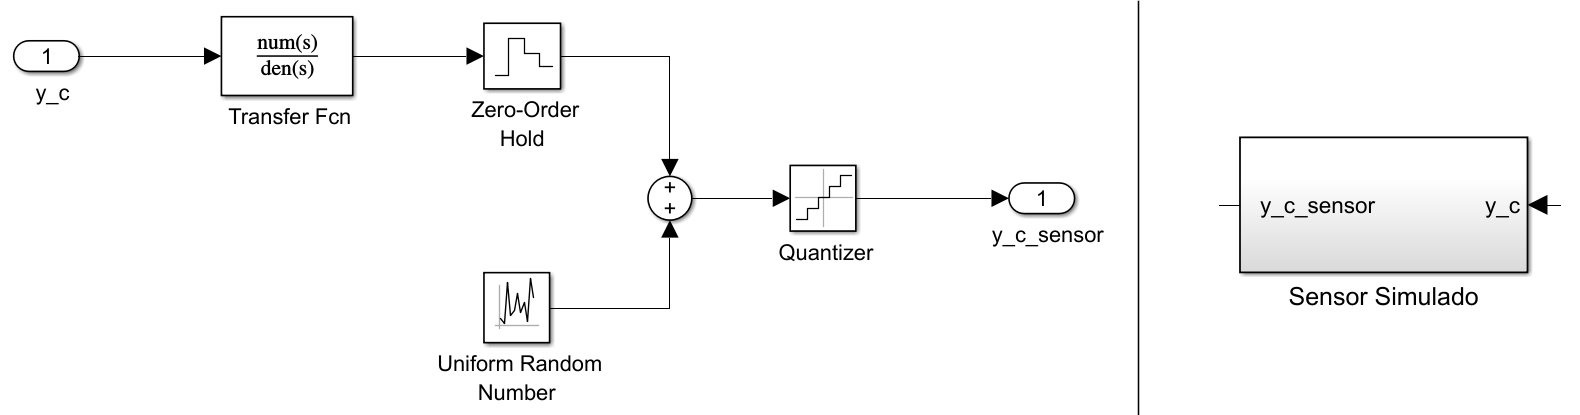
\includegraphics[width=1\linewidth]{figs/bloque_Sensor.png}
    \caption{Bloque sensor de $y_c$}
    \label{fig:bloque_Sensor}
\end{figure}

\subsection{Diseño del observador}

El controlador LQR diseñado previamente requiere realimentación completa de estados. Sin embargo, en una implementación física no resulta práctico medir directamente todas las variables del vector $x(t)$, por este motivo se incorpora un observador de estados, que permite reconstruir el vector completo a partir del modelo de la planta, la entrada aplicada al motor y la medición de $y_c(t)$ disponible del sensor.

El observador continuo se plantea como:

\begin{equation}
\dot{\hat{x}}(t)
=
A\hat{x}(t)+B_cu(t)+L\left(y_s(t)-C_s\hat{x}(t)\right),
\end{equation}

donde $\hat{x}(t)$ es el vector de estados estimado, $u(t)=V_m(t)$, $y_s(t)$ es la medición entregada por el sensor de cremallera y $L$ es la ganancia del observador. El término $y_s(t)-C_s\hat{x}(t)$ es la diferencia entre la posición de cremallera medida y la posición de cremallera estimada por el modelo.

Para calcular $L$ se utiliza un observador de Kalman continuo. En MATLAB se define una matriz de covarianza de proceso $Q$ asociada a incertidumbres del modelo y perturbaciones no representadas, y una covarianza de medición $R$ asociada al ruido del sensor. La ganancia se obtiene mediante:

\begin{equation}
L=\mathrm{lqe}(A,G_w,C_s,Q,R).
\end{equation}

La matriz $G_w$ se adopta como identidad, de modo que las incertidumbres de proceso puedan actuar sobre todos los estados del modelo:

\begin{equation}
G_w=I_7.
\end{equation}

Para $Q$ se utiliza una matriz diagonal cuyos pesos se ajustan para ponderar la confianza relativa en la dinámica de cada estado. En el modelo implementado se adoptaron los siguientes valores:

\begin{equation}
Q=\mathrm{diag}\left(
\begin{bmatrix}
0.1 & 0.1 & 0.1 & 0.01 & 0.01 & 0.01 & 0.01
\end{bmatrix}
\right).
\end{equation}

Aumentar los valores de $Q$ implica asumir mayor incertidumbre en el modelo de proceso, por lo que el observador corrige con mayor rapidez a partir de la medición, aunque puede volverse más sensible al ruido.

Por otro lado, la covarianza de medición se obtiene directamente del modelo de ruido adoptado para el sensor. La desviación estándar equivalente del error uniforme se usa para definir:

\begin{equation}
R=5\,\sigma_{yc}^{2}
=5\left(8.08\times10^{-5}\right)^2
=3.26\times10^{-8}\ \mathrm{m^2}.
\end{equation}

El valor de $R$ aumenta cuando se considera una medición menos confiable, reduciendo el peso de la corrección basada en el sensor. En cambio, un valor menor de $R$ hace que el observador siga con mayor intensidad la medición de $y_c$, aunque también puede volverlo más sensible al ruido, a la cuantización y a la retención de orden cero.

Finalmente, el controlador LQR se implementa utilizando los estados estimados, por lo que la ley de control queda:

\begin{equation}
u(t)=-K_{\mathrm{lqr}}\hat{x}(t)+k_r r(t).
\end{equation}

\begin{figure}[H]
    \centering
    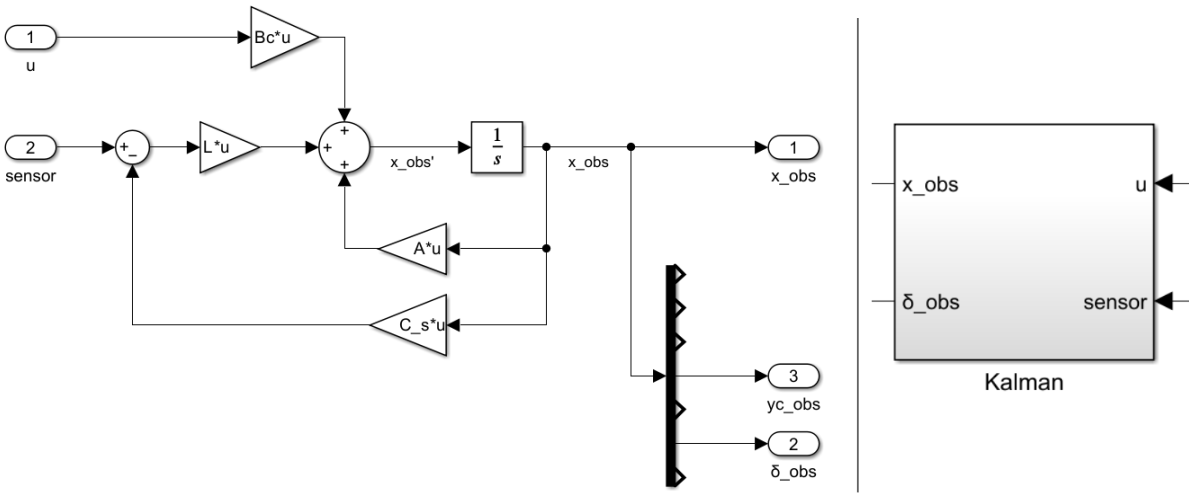
\includegraphics[width=1\linewidth]{figs/bloque_Observador.png}
    \caption{Bloque de Observador en Simulink}
    \label{fig:bloque_Observador}
\end{figure}

Cabe destacar que $\delta_{obs}$ e $y_{c-obs}$ se utilizan únicamente para comparar la estimación con respecto al valor real.

\subsection{Perturbaciones}

Además de la entrada de control $V_m$, el modelo considera perturbaciones mecánicas que actúan sobre la cremallera y sobre el giro de las ruedas. Estas perturbaciones se incorporan mediante la matriz $B_d$ y se agrupan en el vector
\begin{equation}
d(t)=
\begin{bmatrix}
F_f(t) & T_f(t) & T_a(t)
\end{bmatrix}^{T},
\end{equation}
donde $F_f$ representa la fuerza de fricción en la cremallera, $T_f$ el torque de fricción asociado al pivote de la rueda, y $T_a$ el torque de autoalineamiento del neumático.

Los valores nominales de fricción adoptados fueron $F_{f,\mathrm{cte}}=9\ \mathrm{N}$ y $T_{f,\mathrm{cte}}=2\ \mathrm{N\,m}$. Estos valores se tomaron como referencia del trabajo de \hyperlink{ref:azizul-2024}{Azizul et al.}, donde se presenta un modelo completo de vehículo de 14 grados de libertad para sistemas \textit{steer-by-wire}. En una primera aproximación, estas fricciones podrían modelarse mediante funciones signo. Sin embargo, una implementación de ese tipo introduce saltos instantáneos al cambiar el sentido de movimiento, lo cual no resulta representativo de un sistema físico real y puede degradar la simulación numérica.

Por este motivo, en Simulink se implementaron mediante funciones arcotangente:
\begin{equation}
F_f(v_{cr})=
F_{f,\mathrm{cte}}\frac{2}{\pi}
\arctan\left(\frac{v_{cr}}{v_{\epsilon,cr}}\right),
\end{equation}
\begin{equation}
T_f(\psi)=
T_{f,\mathrm{cte}}\frac{2}{\pi}
\arctan\left(\frac{\psi}{\omega_{\epsilon,f}}\right),
\end{equation}
donde $v_{cr}$ es la velocidad de la cremallera y $\psi=\dot{\delta}$ es la velocidad angular de la rueda. En la simulación se utilizaron $v_{\epsilon,cr}=10^{-4}\ \mathrm{m/s}$ y $\omega_{\epsilon,f}=10^{-4}\ \mathrm{rad/s}$. Con esta formulación, para velocidades suficientemente grandes el valor tiende a $\pm F_{f,\mathrm{cte}}$ o $\pm T_{f,\mathrm{cte}}$, mientras que alrededor de cero se obtiene una transición continua.

El torque de autoalineamiento $T_a$ aparece cuando el neumático desarrolla fuerza lateral (representada en la figura \ref{fig:fuerza_resultante_lateral}). Debido a la deformación de la huella de contacto, la resultante lateral no actúa exactamente sobre el centro geométrico de la rueda, sino con un brazo efectivo conocido como \textit{pneumatic trail}. Esto genera un torque que tiende a alinear la rueda con la dirección de avance. La relación física utilizada como base fue la indicada por \hyperlink{ref:rill-first-order}{Rill}, donde el torque autoalineante puede interpretarse como el producto entre la fuerza lateral y dicho brazo efectivo.

\begin{figure}[H]
    \centering
    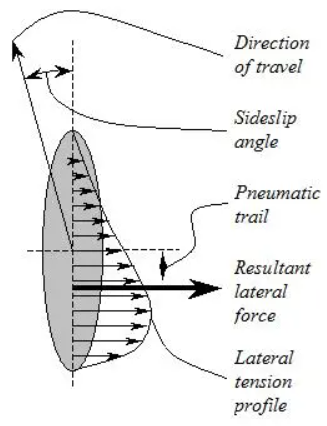
\includegraphics[width=0.3\linewidth]{figs/fuerza_resultante_lateral.png}
    \caption{Fuerza resultante lateral debido a una rotación de la rueda en sentido horario}
    \label{fig:fuerza_resultante_lateral}
\end{figure}



En este trabajo no se modela el neumático con un modelo dinámico completo. En cambio, se estimó $T_a$ por rueda a partir de un modelo bicicleta en régimen estacionario. Primero se calcula el ángulo de deriva delantero $\alpha_f$ (\textit{sideslip angle} en la figura \ref{fig:fuerza_resultante_lateral}) a partir de $\delta(t)$ y de la velocidad longitudinal del vehículo. Luego se estima la fuerza lateral por rueda con una saturación suave:
\begin{equation}
F_{y,\mathrm{wheel}}=
F_{y,\max}\tanh\left(\frac{C_{f,\mathrm{wheel}}\alpha_f}{F_{y,\max}}\right).
\end{equation}
Finalmente, el brazo efectivo se aproxima mediante
\begin{equation}
t_{\mathrm{eff}}=
t_0\,e^{-k_{\alpha}|\alpha_f|}
\frac{1}{1+\left(V_x/V_t\right)^2},
\end{equation}
y el torque autoalineante queda dado por
\begin{equation}
T_a=F_{y,\mathrm{wheel}}\,t_{\mathrm{eff}}.
\end{equation}
En el modelo se adoptaron $t_0=0.08\ \mathrm{m}$, $k_{\alpha}=8$, mientras que la velocidad $V_t\ \mathrm{[m/s]}$ puede ser variable. Para velocidades menores a $0.5\ \mathrm{m/s}$ se impone $T_a=0$, ya que en una maniobra prácticamente detenida no se genera una fuerza lateral estacionaria representativa. Esta simplificación permite introducir el efecto restaurador principal del neumático sin aumentar de forma significativa la complejidad del modelo.

\subsection{Resultados}

A continuación se muestra una imagen con la disposición de los bloques que conforman la simulación en Simulink:

\begin{figure}[H]
    \centering
    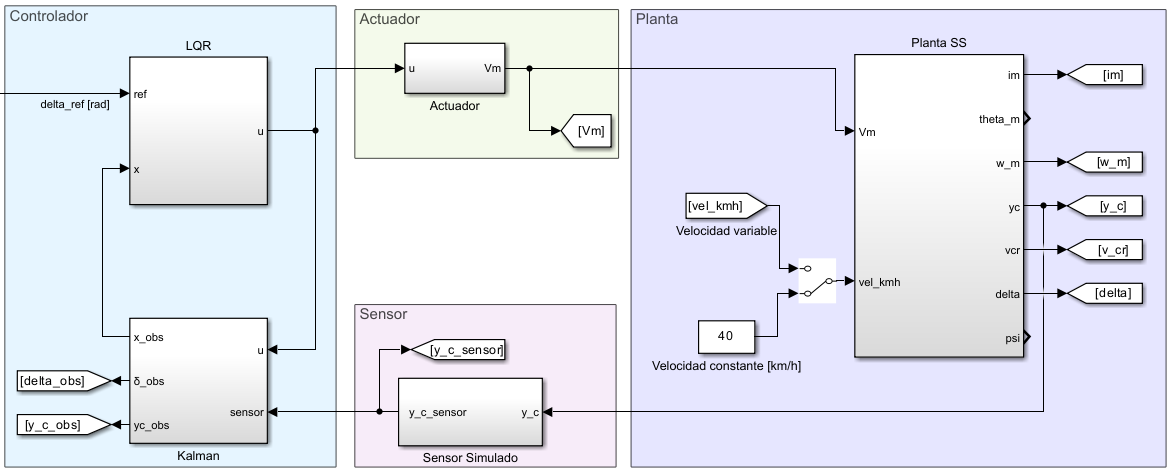
\includegraphics[width=1\linewidth]{figs/Simulink_final.png}
    \caption{Interconexión de bloques en Simulink}
    \label{fig:Simulink_final}
\end{figure}

\subsubsection{Referencia trapezoidal de \texorpdfstring{$35^\circ$}{35°} a \texorpdfstring{$40\ \mathrm{km/h}$}{40 km/h}}

Para evaluar el sistema se utiliza una referencia trapezoidal de $35^\circ$, en lugar de una entrada escalón. Esta forma de consigna resulta más representativa de una entrada generada por un volante y evita exigir aceleraciones instantáneas al actuador, lo cual reduce los picos de corriente y torque del motor durante el inicio de la maniobra.

\begin{figure}[H]
    \centering
    \begin{subfigure}[t]{0.49\linewidth}
        \centering
        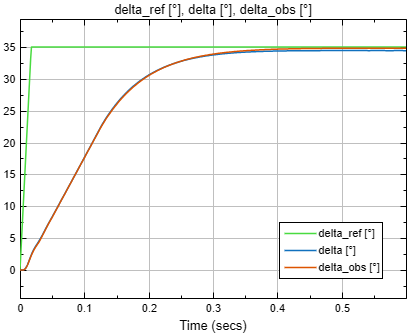
\includegraphics[width=\linewidth]{figs/rtaDelta_entradaTrapezoidal.png}
        \caption{Respuesta completa.}
        \label{fig:respuesta_trapezoidal_completa}
    \end{subfigure}
    \hfill
    \begin{subfigure}[t]{0.49\linewidth}
        \centering
        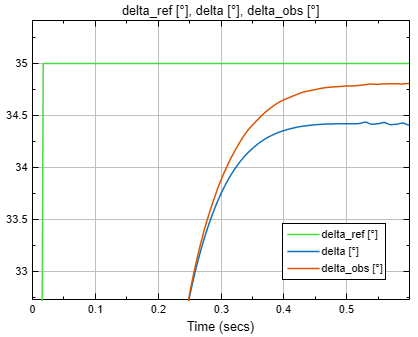
\includegraphics[width=\linewidth]{figs/rtaDelta_entradaTrapezoidalZoom.png}
        \caption{Detalle de la respuesta.}
        \label{fig:respuesta_trapezoidal_zoom}
    \end{subfigure}
    \caption{Respuesta $\delta(t)$ ante una referencia trapezoidal de $35^\circ$.}
    \label{fig:respuesta_trapezoidal}
\end{figure}

En la figura \ref{fig:respuesta_trapezoidal} se observa que el sistema sigue la forma general de la referencia, aunque queda un error estacionario cercano a $0.4^\circ$ respecto de los $35^\circ$ solicitados. Este error aparece porque el ensayo incluye perturbaciones sostenidas sobre la rueda, en particular el torque autoalineante del neumático. La señal $\delta_{\mathrm{obs}}$ estimada por el observador sigue la tendencia de $\delta$, pero queda levemente por encima del ángulo real. Esta diferencia es coherente con la arquitectura adoptada: el observador reconstruye el estado completo a partir de la medición de la posición de cremallera $y_c$, pero no mide directamente el ángulo de rueda. Por lo tanto, ante perturbaciones externas aplicadas sobre la rueda puede aparecer un sesgo entre la estimación de $\delta$ y el valor real.

Durante esta maniobra, el desplazamiento de la cremallera asociado al giro de $35^\circ$ es de aproximadamente $70\ \mathrm{mm}$. Considerando que la respuesta se completa en el orden de $0.55\ \mathrm{s}$, se obtiene una velocidad media equivalente cercana a $127\ \mathrm{mm/s}$. Este valor se encuentra en el mismo orden de magnitud que la velocidad lineal declarada para el \hyperlink{ref:schaeffler-rwa}{Road Wheel Actuator de Schaeffler}, que es de hasta $140\ \mathrm{mm/s}$.

\subsubsection{Perturbaciones y esfuerzo de actuación}

\begin{figure}[H]
    \centering
    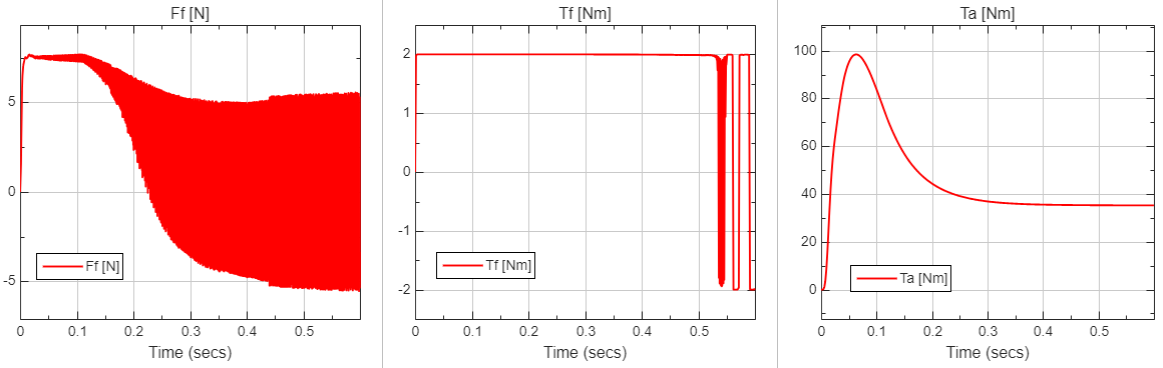
\includegraphics[width=1\linewidth]{figs/perturbaciones_entradaTrapezoidal.png}
    \caption{Perturbaciones $F_f(t)$, $T_f(t)$ y $T_a(t)$ ante referencia trapezoidal de $35^\circ$}
    \label{fig:perturbaciones_trapezoidal}
\end{figure}

En la figura \ref{fig:perturbaciones_trapezoidal} se muestra la evolución de las perturbaciones aplicadas al modelo. El torque autoalineante $T_a$ presenta un pico inicial durante el transitorio y luego converge a un valor constante menor a $40\ \mathrm{N\,m}$. Esta carga sostenida explica el error estacionario observado en la figura \ref{fig:respuesta_trapezoidal}: el controlador LQR no posee acción integral y, al existir una perturbación constante sobre la rueda, el equilibrio final se alcanza con una pequeña diferencia entre $\delta$ y $\delta_{ref}$.

No se incorporó acción integral en el controlador final porque, en una aplicación de dirección, la referencia es generada de manera continua por el conductor o por un sistema de asistencia, y no suele permanecer fija durante largos intervalos como en un problema clásico de regulación. Además, en las pruebas realizadas se implementó una variante LQRI, pero no resultó efectiva para eliminar completamente el error estacionario ante perturbaciones sostenidas. Esto se debe a que el integrador fue diseñado sobre el error de $\delta$, mientras que en la arquitectura propuesta la medición disponible para el observador es la posición de cremallera $y_c$. Ante perturbaciones externas aplicadas sobre la rueda puede existir una diferencia estacionaria entre $y_c$ y $\delta$ debido a la elasticidad del sistema mecánico.

Para que un LQRI resulte adecuado en esta arquitectura sería necesario medir directamente $\delta$ o, alternativamente, diseñar un observador de estado aumentado que estime las perturbaciones externas constantes. También debería incorporarse una estrategia de \textit{anti-windup}, ya que el actuador se encuentra limitado a $\pm48\ \mathrm{V}$ y, cuando trabaja cerca de la saturación, el integrador puede acumular error aunque el sistema no pueda aplicar la tensión demandada. Por estos motivos, en este trabajo se priorizó una respuesta rápida y limitada por las capacidades físicas del actuador, aceptando un pequeño error estacionario ante perturbaciones sostenidas.

Las fricciones $F_f$ y $T_f$ fueron implementadas mediante funciones arcotangente para evitar saltos discontinuos entre valores positivos y negativos. Por este motivo, cuando el sistema se aproxima al equilibrio y la velocidad cambia de signo por pequeñas correcciones del controlador, las fricciones oscilan alrededor de su cambio de signo.

Analizando entonces los gráficos de perturbaciones, se observa que el torque autoalineante $T_a$ es la perturbación dominante durante la maniobra. Para este caso particular de referencia trapezoidal de $35^\circ$, su pico transitorio puede alcanzar valores muy superiores al torque de fricción $T_f$.

\begin{figure}[H]
    \centering
    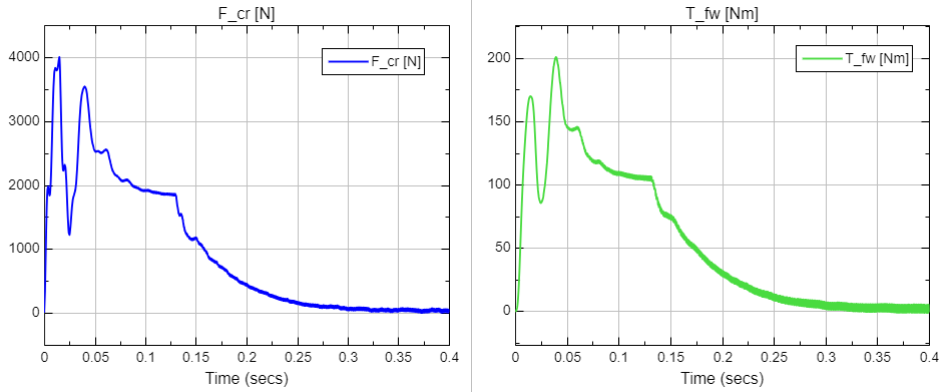
\includegraphics[width=1\linewidth]{figs/Esfuerzo_entradaTrapezoidal.png}
    \caption{Fuerza $F_{cr}$ y torque $T_{fw}$ efectivos aplicados sobre cremallera y rueda, respectivamente.}
    \label{fig:esfuerzo_trapezoidal}
\end{figure}

Como puede verse en la figura \ref{fig:esfuerzo_trapezoidal}, la fuerza $F_{cr}$ aplicada sobre la cremallera y el torque $T_{fw}$ aplicado sobre la rueda son significativamente superiores a las perturbaciones modeladas. Esto indica que la arquitectura mecánica elegida tiene la capacidad de generar las fuerzas y torques suficientes como para poder hacer que el sistema siga a la referencia a pesar de perturbaciones de gran magnitud como $T_a$.

\subsubsection{Validación de operación del motor}

\begin{figure}[H]
    \centering
    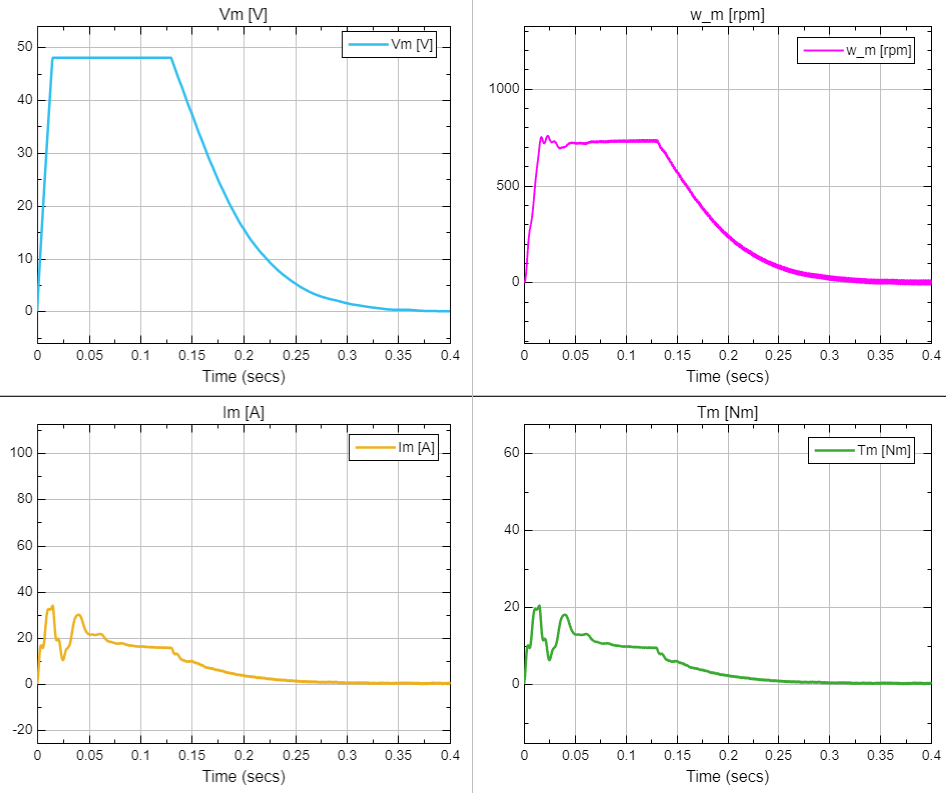
\includegraphics[width=1\linewidth]{figs/motor_entradaTrapezoidal.png}
    \caption{Variables eléctricas y mecánicas del motor ante referencia trapezoidal de $35^\circ$}
    \label{fig:motor_respuesta_trapezoidal}
\end{figure}

\begin{table}[H]
\small
\centering
\caption{Validación del motor ante referencia trapezoidal de $35^\circ$}
\label{tab:validacion_motor_trapezoidal}
\begin{tabular}{l c c}
\toprule
\textbf{Magnitud} & \textbf{Valor obtenido} & \textbf{Límite admisible} \\
\midrule
$\max(|V_m|)$ & $48\ \mathrm{V}$ & $48\ \mathrm{V}$ \\
$\max(|i_m|)$ & $42.6\ \mathrm{A}$ & $70\ \mathrm{A}$ \\
$i_{m,\mathrm{RMS}}$ & $13.5\ \mathrm{A}$ & $30\ \mathrm{A}$ \\
$\max(|T_m|)$ & $25.6\ \mathrm{N\,m}$ & $40\ \mathrm{N\,m}$ \\
$T_{m,\mathrm{RMS}}$ & $8.1\ \mathrm{N\,m}$ & $18\ \mathrm{N\,m}$ \\
$\max(|\omega_m|)$ & $780\ \mathrm{rpm}$ & $800\ \mathrm{rpm}$ \\
\bottomrule
\end{tabular}
\end{table}

Como se observa en la tabla \ref{tab:validacion_motor_trapezoidal}, los valores de tensión, corriente, torque y velocidad se mantienen dentro de los límites admisibles. En pruebas realizadas utilizando referencia escalón, el pico de corriente podía alcanzar valores de casi $100\ \mathrm{A}$ y velocidades de $1200\ \mathrm{rpm}$; de allí la importancia de usar entradas trapezoidales para hacer la validación del motor.

Como puede observarse en la gráfica de $V_m$, el controlador LQR fue ajustado para aprovechar al máximo la capacidad disponible del actuador, incluso cuando esto implica alcanzar la saturación de tensión. Este criterio de diseño se adoptó porque el sistema está orientado a vehículos tripulados, donde se prioriza la seguridad y resulta necesario que el conductor pueda realizar maniobras rápidas y precisas ante situaciones de emergencia.

\subsubsection{Caso particular a \texorpdfstring{$100\ \mathrm{km/h}$}{100 km/h}}

Como caso particular, se repitió el análisis con una velocidad longitudinal de $100\ \mathrm{km/h}$. Este escenario no se adopta como condición nominal de validación, sino como una prueba para interpretar el comportamiento del modelo de torque autoalineante fuera de la zona de maniobra moderada. En esa condición, para una referencia de $35^\circ$, el ángulo de deriva resultante es mucho más severo. Dentro de la simplificación adoptada para el neumático, la fuerza lateral alcanza rápidamente su zona de saturación y el \textit{pneumatic trail} efectivo disminuye hasta valores muy pequeños. Por ese motivo, el torque autoalineante presenta un pico transitorio y luego cae prácticamente a cero. Este comportamiento no debe interpretarse como ausencia de esfuerzos reales en el neumático, sino como una consecuencia del modelo simplificado utilizado para representar la pérdida de capacidad restauradora a grandes ángulos de deriva y alta velocidad. Ante dicha situación, el usuario notaría falta de agarre y que el vehículo se va recto por más que el volante y las ruedas estén rotados. A este fenómeno se lo conoce como subviraje o \textit{understeer}.

\begin{figure}[H]
    \centering
    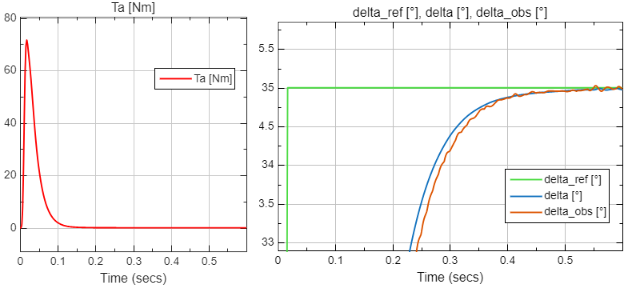
\includegraphics[width=0.9\linewidth]{figs/rta_100kmh.png}
    \caption{Torque autoalineante $T_a(t)$ y respuesta $\delta(t)$ ante referencia trapezoidal de $35^\circ$ a $100\ \mathrm{km/h}$}
    \label{fig:rta_100kmh}
\end{figure}

En la figura \ref{fig:rta_100kmh} puede observarse que al hacerse nulo $T_a$, $\delta$ converge a la referencia sin un error estacionario apreciable. 

\subsubsection{Simulación en Unity}

Para validar el comportamiento del modelo matemático con entradas más cercanas a una maniobra real, se decidió probar el sistema utilizando señales generadas desde un volante Logitech G923. En esta prueba, el modelo de control y actuación continúa ejecutándose en Simulink, mientras que las variables principales de la simulación se envían en tiempo real hacia Unity mediante comunicación UDP.

En el entorno de Unity se utiliza como base el controlador físico \hyperlink{ref:prometeo-car-controller}{\textit{PROMETEO: Car Controller}}. En su implementación original, el controlador recibe una entrada asociada al giro del volante y la transforma internamente en una consigna de dirección para las ruedas, incorporando además un retardo para representar el atraso físico entre la acción sobre el volante y la respuesta de giro de los neumáticos. En este trabajo, dicha dinámica ya se encuentra representada en el modelo desarrollado en Simulink, por lo que no resulta necesario volver a incorporarla dentro del entorno de Unity. Por este motivo, se modificó el controlador PROMETEO para aplicar directamente $\delta(t)$ como ángulo de giro a las ruedas delanteras. De esta manera, el vehículo no es rotado artificialmente, sino que su movimiento resulta de la interacción física entre las ruedas y el suelo dentro del motor de física de Unity, de forma análoga a lo que ocurre en un vehículo real.

Esta prueba permite verificar cualitativamente que la respuesta del controlador no solo sigue de manera coherente la referencia en las gráficas de Simulink, sino que además produce una maniobra familiar para el usuario. En el siguiente enlace puede verse un video donde se muestra una prueba de la interacción entre ambos sistemas, además de gráficas mínimas para mostrar el seguimiento de la respuesta y parámetros del motor en tiempo real:

\begin{center}
\href{https://www.youtube.com/watch?v=QAsnqMuFXuQ}{Video de validación en Unity}
\end{center}

\begin{figure}[H]
    \centering
    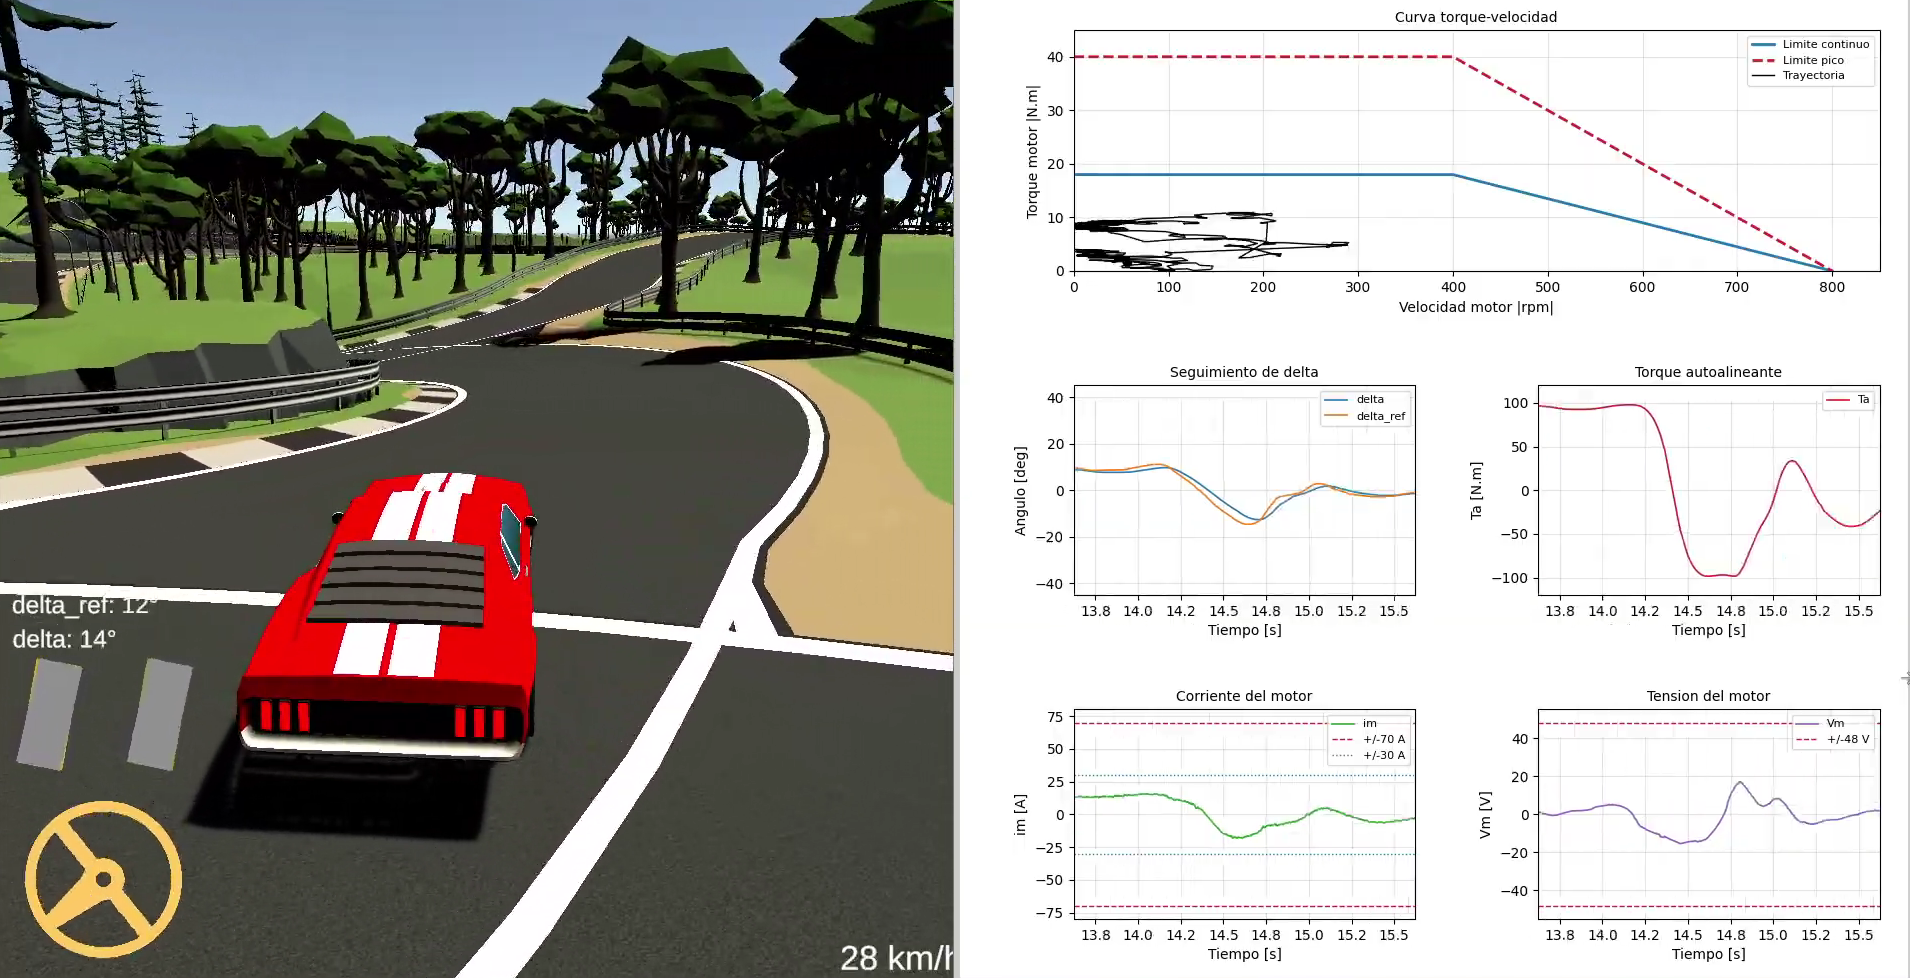
\includegraphics[width=1\linewidth]{figs/Unity.png}
    \caption{Captura del video mostrando el vehículo respondiendo a la referencia de dirección generada por volante.}
    \label{fig:unity}
\end{figure}

El código completo del proyecto, incluyendo el modelo de Simulink, el informe y los scripts auxiliares utilizados para la visualización en tiempo real, se encuentra disponible en el siguiente repositorio:

\begin{center}
\href{https://github.com/RodriAleo/CyS_Steering_By_Wire/tree/main}{GITHUB: CyS\_Steering\_By\_Wire}
\end{center}

\section{Conclusiones}

En el trabajo desarrollado los resultados muestran que el sistema puede seguir referencias de dirección exigentes y que el actuador seleccionado opera dentro de límites razonables cuando las consignas se plantean de forma realista. Además, la simulación con perturbaciones permitió verificar que el actuador cuenta con margen suficiente para contrarrestar fricción y torque autoalineante, aunque también evidenció la aparición de un pequeño error estacionario cuando el torque autoalineante se mantiene como perturbación sostenida.

La validación adicional en Unity permitió comprobar de manera cualitativa que la salida del modelo no solo es consistente en las gráficas de Simulink, sino que también produce una respuesta vehicular coherente al aplicarse sobre un modelo físico interactivo. Esta prueba resulta útil como paso intermedio entre la simulación puramente matemática y una implementación experimental, ya que permite observar el efecto del ángulo de rueda calculado sobre la dinámica visible del vehículo.

Como trabajo futuro, un paso natural sería implementar el controlador discretizado y probarlo mediante una plataforma de \textit{hardware-in-the-loop}, incorporando tiempos de muestreo, comunicación y procesamiento más representativos de una implementación real. También sería conveniente ajustar con mayor precisión los parámetros mecánicos de la transmisión, la cremallera y el enlace con las ruedas, con el objetivo de obtener fuerzas y torques más cercanos a los de un actuador real. Finalmente, se debería mejorar el modelo de perturbaciones para incluir situaciones no contempladas en este estudio, como el esfuerzo requerido para girar el neumático cuando el vehículo está detenido o cuando existe rotación de la rueda sobre su propio eje sin avance longitudinal significativo.

\section{Referencias}
\addcontentsline{toc}{section}{Referencias}

\subsection*{Parámetros de planta, actuador, perturbaciones y sensor}

\begin{itemize}
    \item \hypertarget{ref:recursos-catedra}{}\textbf{Recursos aportados por la cátedra}. Repositorio con material de apoyo, consignas, guías y recursos complementarios provistos durante el cursado de la asignatura para el desarrollo del trabajo. Disponible en: \url{https://github.com/carloshernangarrido/control}.
    
    \item \hypertarget{ref:azizul-2024}{}\textbf{M. A. Azizul, F. Ahmad, J. Karjanto, M. H. Che Hasan y S. Sulaiman, \textit{Modelling, Simulation and Testing of Steer-by-Wire System with Variable Steering Ratio Control Strategy in 14-DOF Full Vehicle Model}}. \url{https://doi.org/10.15282/ijame.21.4.2024.5.0908}.
    
    \item \hypertarget{ref:taher-2025}{}\textbf{Taher Sachit Taher et al., \textit{Improving the Performance of Steering by Wire Using a Model Predictive Controller Enhanced with Particle Swarm Optimisation}}. \url{https://doi.org/10.22153/kej.2025.01.002}.
    
    \item \hypertarget{ref:bosch-48v}{}\textbf{Bosch, \textit{48 V battery}}. Referencia sobre el uso de redes y baterías de $48\ \mathrm{V}$ en vehículos modernos y sistemas mild-hybrid. \url{https://www.bosch-mobility.com/en/solutions/batteries/48-v-battery/}.

    \item \hypertarget{ref:mosrac-u13060}{}\textbf{Mosrac, \textit{U130 Series Frameless Direct Drive Torque Motors}}. Catálogo web utilizado como referencia para el motor equivalente Mosrac U13060 de $48\ \mathrm{V}$. \url{https://www.mosrac.com/products/frameless-direct-drive-torque-motors/u130-series.html}.  

    \item \hypertarget{ref:mlx90513}{}\textbf{Melexis, \textit{MLX90513 Inductive Position Sensor Interface IC}}. \url{https://www.melexis.com/-/media/files/documents/datasheets/mlx90513-datasheet-melexis.pdf}.

    \item \hypertarget{ref:schaeffler-rwa}{}\textbf{Schaeffler, \textit{Road Wheel Actuator}}. \url{https://www.schaeffler.us/us/products-and-solutions/powertrain-chassis/road-wheel-actuator/}.

    \item \hypertarget{ref:prometeo-car-controller}{}\textbf{Unity Asset Store, \textit{PROMETEO: Car Controller}}. \url{https://assetstore.unity.com/packages/tools/physics/prometeo-car-controller-209444}.
\end{itemize}

\subsection*{Modelo de torque autoalineante}

\begin{itemize}
    \item \hypertarget{ref:rill-first-order}{}\textbf{Georg Rill, \textit{First Order Tire Dynamics}}. Disponible en: \url{https://www.researchgate.net/publication/317036997_First_Order_Tire_Dynamics}. De esta fuente se tomó la relación física básica entre torque autoalineante y fuerza lateral, expresada como $T_S = c_o F_y$, donde $c_o$ representa el \textit{pneumatic trail}. Esta idea se utilizó como base para escribir $T_a$ como producto entre fuerza lateral y brazo efectivo del neumático, con signo restaurador.

    \item \textbf{ScienceDirect Topics, \textit{Aligning Torque}}. Disponible en: \url{https://www.sciencedirect.com/topics/engineering/aligning-torque}. De esta fuente se extrajo el comportamiento cualitativo esperado del torque autoalineante en neumáticos reales: crecimiento aproximadamente lineal para ángulos de deriva pequeños, aparición de un máximo a bajos ángulos de deriva y disminución posterior al aumentar el deslizamiento lateral. También se utilizó para justificar que el \textit{pneumatic trail} disminuye cuando crece el ángulo de deriva.

    \item \textbf{ScienceDirect Topics, \textit{Brush Model}}. Disponible en: \url{https://www.sciencedirect.com/topics/engineering/brush-model}. De esta fuente se tomó la interpretación mecánica del origen del torque autoalineante mediante la distribución no simétrica de esfuerzos en la huella de contacto, y la observación de que un valor más realista del \textit{trail} a bajo deslizamiento puede aproximarse como $t \approx 0.5\,a$, siendo $a$ la semilongitud de la huella. Este criterio se utilizó como referencia para contrastar el valor de \textit{trail} adoptado en el modelo simplificado.

    \item \textbf{Turan Alp Arslan et al., \textit{Investigation of the Effects of Axle Load on Tyre Behaviour in Vehicles}}. Disponible en: \url{https://www.researchgate.net/publication/365781200_Investigation_of_the_Effects_of_Axle_Load_on_Tyre_Behaviour_in_Vehicles}. De este trabajo se tomaron supuestos geométricos y de carga para un neumático individual 205/55R16, en particular el uso de una muestra de una sola rueda, la presión de inflado del orden de $220.632\ \mathrm{kPa}$ y la relación entre ancho efectivo de huella y ancho del neumático. Estos datos se usaron en el análisis en Python para estimar una longitud de huella razonable por rueda y, a partir de ella, un orden de magnitud plausible del \textit{pneumatic trail}.

    \item \textbf{Hsu, Laws y Gerdes, \textit{Estimation of Tire Slip Angle and Friction Limits Using Steering Torque}}. Disponible en: \url{https://www.researchgate.net/publication/224603533_Estimation_of_Tire_Slip_Angle_and_Friction_Limits_Using_Steering_Torque}. De esta referencia se utilizó la idea de que la información del torque de dirección está fuertemente vinculada con la evolución del \textit{pneumatic trail}, y que la caída de dicho \textit{trail} es un indicador físicamente consistente del acercamiento a la saturación lateral del neumático.
\end{itemize}

\end{document}
